


\chapter{Calibration procedure}
\label{chapter:calibration}

%\section{Review of level0 data}
%The thermal and electrical environment of a satellite may cause
%receiver instabilities, which must be compensated. Whereas ground
%based systems may have relatively stable gain but changing system
%temperature due to unstable weather conditions, the Odin satellite
%shows the opposite behaviour: stable noise figures in spite of cyclic
%gain variations during one orbit.

%\section{Measurement sequence and radiance calibration process}


\section{Processing pipeline}

Raw science and house-keeping data are downloaded at
Esrange and transferred to a data archive housed by the Parallel
Data Centre (PDC) at the Royal Institute of Technology (KTH)
in Stockholm. The data processing for the calibration \smr\
measurements are performed at the Dept. of Earth and Space
Sciences at Chalmers University of Technology (CTH) in Gothenburg.
A file system at CTH is synchronized with the Level0-file archive 
at KTH. The kTH archive also contains files with reconstructed attitude
information.  Science and house keeping data within those files
are imported into Level0 tables of an Odin calibration database
( a postgresql database). 
Dedicated algorithms to process and combine new Level0 to Level1b
data are executed on a regular basis, and are described in this
chapter. Level1B data are stored in tables of the Odin calibration database.  
How to access the Level1B data and the its format is described
in Chapter 3.

\lcomment{BR}{shoud this be included?}



\section{Important aspects for calibration}


The definition of a scan (in calibration version 8) is based
on the measurement sequence. A scan consists of all type of signals and data that
where recorded from the first 'load signal' (when such are collected) until the
next sequence of 'load signals'. In practise, this is equivalent to all 
measurements collected between the lower turning point and upper turning point
(or vice versa) of the limb-scanning motion.

An important aspect for the calibration is to take into account
that the main beam signal is always at a higher level than the cold sky signal,
due to thermal emission from a baffle, that only affect the main beam signal.

It has also turned out out that a slight imbalance between signal and 
reference phase introduces instabilities seen as low-level ripple 
in calibrated atmospheric spectra, if not taken into account. 

frequency calibration

pointing?


%the spectrometer passbands. This ripple is stable in the IF band,
%and can be measured towards a blank region of the sky and subsequently
%be subtracted from target spectra.

%A scan is then defined as all measurements collected between two hot
%load signals, which in practise is equivalent to all measurements
%collected between the lower turning point and upper turning point
%(or vice versa) of the limb-scanning motion. Table 2
%lists the scanning range of the three main scanning modes used.




\section{Radiometric calibration algorithm}

\subsection{Auto-correlator data}

Data from the ACs must be transformed to spectra in the frequency domain
prior to the radiometric calibration. 
In the spectrometer hardware, the input signal is quantized into three levels: 
high positive, high negative and low amplitude. The input signal is furthermore delayed, 
cross multiplied and integrated to obtain a distorted measure of the auto-correlation function of the 
input signal \(s(t)\).
Accurate quantization correction require accurate knowledge of the threshold
levels used at quantization.
The Odin correlators provide monitor channels to check the
assumption of equal absolute values of the positive and negative threshold levels.
And only when this condition is fulfilled the data will be processed.
The estimation of the true correlation \(\rho\) from the measured modified correlation 
coefficient \(r\) at lag \(\tau\) is then achieved by performing a quantisation correction using 
Kulkarni and Heiles approximation described in \citet{ohlberg:theod:03}.

The fourier transform of the auto correlation function is then the
power spectral density, or a spectrum in the frequency domain. 
But before the fourier transform is calculated a Hanning smoothing is
applied, which gives that the obtained resolution of the spectra is 2\,MHz,
although the channel spacing is 1\,MHz.


\subsection{Intensity calibration basics}

The intensity calibration of \smr\ is performed by using
information from three type of signals, i.e. the sky beam signal
(\(c_{s}\)),
the load signal (\(c_{l}\)), and the main beam signal (\(c_{a}\)).
The calibration scheme is based on the assumption that the 
digital value (e.g. \(c_{a,i}\)) read out from channel \(i\) of the 
spectrometer and 
normalised by division by integration time, is proportional to the
observed signal. The contributions to the signals 
can be expressed as:
\begin{equation}
c_{a,i}=g_{i}\left(\eta_{a} T_{a,i}+(1-\eta_{a})T_{amb,i}+T_{rec,i}\right),
\end{equation}
\begin{equation}
\label{eq:skybeam}
c_{s,i}=g_{i}\left(T_{s,i}+T_{rec,i}\right),
\end{equation}
\begin{equation}
c_{l,i}=g_{i}\left(T_{l,i}+T_{rec,i}\right),
\end{equation}
where \(g_{i}\) is the receiver gain, \(\eta_{a}\) is the main beam
efficiency (it is assumed that beam efficiences for 
both the sky beam and load signals are unity), 
\(T_{amb,i}\) is the receiver ambient temperature,
and \(T_{rec,i}\) is the receiver noise temperature.
\(T_{a,i}\), \(T_{s,i}\), and \(T_{l,i}\) are the antenna temperature,
cosmic background temperature, and load temperature all expressed
as equivalent Rayleigh-Jeans brightness temperatures (Tb).

Around 500 GHz \(T_{s,i}\) is only 0.003 K, and for Odin-SMR
\(T_{rec,i}\) is in the order of 3000 K, thus Eq.~\ref{eq:skybeam} gives
to a very high degree that
\begin{equation}
\label{eq:trec}
T_{rec,i}=\frac{c_{s,i}}{g_{i}}.
\end{equation}
\(g_{i}\) can be obtained from the difference between \(c_{l,i}\) and
 \(c_{s,i}\), i.e.
\begin{equation}
\label{eq:gain}
g_{i}=\frac{c_{l,i}-c_{s,i}}{T_{l,i}-T_{s,i}}.
\end{equation}
By combining Eq.~\ref{eq:trec} and~\ref{eq:gain} we obtain
\begin{equation}
\label{eq:trec2}
T_{rec,i}=\frac{c_{s,i}({T_{l,i}-T_{s,i}})}{c_{l,i}-c_{s,i}}.
\end{equation}
\(T_{a,i}\) can be obtained from the difference between between
\(c_{a,i}\) and \(c_{s,i}\), i.e.
\begin{eqnarray}
\label{eq:ta}
T_{a,i} &=& \frac{1}{\eta_{a}}\left(\frac{c_{a,i}-c_{s,i}}{g_{i}}+T_{s,i}-(1-\eta_{a})T_{amb}\right) \nonumber\\
 &=& \frac{1}{\eta_{a}}\left( \left(\frac{c_{a,i}}{c_{s,i}}-1\right)T_{rec,i}+T_{s,i}-T_{sp}\right), 
\end{eqnarray}
where the spill over contribution (\(T_{sp}\)): 
\begin{equation}
\label{eq:tspill1}
T_{sp}=(1-\eta_{a})T_{amb}
\end{equation}
is due to the difference
in the efficiences for the main beam and sky beam.
The main beam intercepts with the baffle and is therefore
smaller than unity, whereas the sky beam efficiency is assumed to be unity. 
For measurements at tangent altitude above the atmosphere
\(T_{a,i}\)=\(T_{s,i}\). Thus, we have that for these measurements
to a very good approximation
\begin{equation}
\label{eq:tspill2}
T_{sp,i}= \left(\frac{c_{a,i}}{c_{s,i}}-1\right)T_{rec,i}+T_{s,i}.
\end{equation}
Combining Eq.~\ref{eq:tspill1} and~\ref{eq:tspill2} gives that
\begin{equation}
\label{eq:eta}
\eta_{a}=1-\frac{T_{sp}}{T_{amb}}=1-\frac{\left(\frac{c_{a,i}}{c_{s,i}}-1\right)T_{rec,i}+T_{s,i}}{T_{amb}}.
\end{equation}

\subsection{Low level ripple}

Equation~\ref{eq:ta} can be thought of as the main intensity
calibration equation for the Odin  calibration scheme
In the derivation of Eq.~\ref{eq:ta}
the reference signals are assumed to be ''clean''.
Ripple on the sky and load signals will
result in undesired feature in calibrated
spectra, if not taking into account.
%This section describes how 
%ripple on those signals
%can be taking into account in the calibration process.
The sensitivity on calibrated \(T_{a,i}\) to ripple on the reference signals,
or to small perturbations on \(T_{s,i}\) and \(T_{l,i}\) are:
\begin{equation}
\frac{dT_{a,i}}{dT_{s,i}}=\frac{1}{\eta_{a}}\left(1-\frac{c_{a,i}-c_{s,i}}{c_{l,i}-c_{s,i}}\right)\approx \frac{1}{\eta_{a}}\left(1-\frac{T_{a,i}}{T_{l,i}}\right)
\end{equation}
and
\begin{equation}
\frac{dT_{a,i}}{dT_{l,i}}=\frac{1}{\eta_{a}}\left(\frac{c_{a,i}-c_{s,i}}{c_{l,i}-c_{s,i}}\right)\approx \frac{1}{\eta_{a}}\left(\frac{T_{a,i}}{T_{l,i}}\right).
\end{equation}
Thus, the sensitivity is linearly proportional to \(T_{a,i}\).
When \(T_{a,i}\) is 0 K or close to 0 K (as it is for measurements at high
tangent altitudes) the sensitivity to perturbations on
the sky beam signal is at its maximum.
Perturbations on the load signal, on the other hand, has then pratically
no impact on \(T_{a,i}\).
When \(T_{a,i}\) is equal to the load temperature (but it never is)
the situation is the reversed.

A model for the removal of the effects of ripple on the reference signals
on estimated \(T_{a,i}\) (from Eq.~\ref{eq:ta}) to achieve a new
better estimate \(T^{'}_{a,i}\) of the antenna temparture then reads
\begin{equation}
\label{correction}
T^{'}_{a,i}=T_{a,i}-\frac{1}{\eta_{a}}\left(1-\frac{T_{a,i}}{T_{l,i}}\right) s_{0,i}-
 \frac{1}{\eta_{a}}\left(\frac{T_{a,i}}{T_{l,i}}\right) s_{1,i},
\end{equation}
where \(s_{0,i}\) and \(s_{1,i}\) can be seen as spectra that contain
the ripple induced features for \(T_{a,i}\)=0 K and \(T_{a,i}\)=load temperature,
respectively.

\subsection{Intensity calibration scheme} 

The intensity calibration scheme can be divided into two parts. The first part can be
seen as a scan based calibration scheme, where the Equations of Sect. ? are applied.
The second part takes into account of ripple? on reference signals, and uses the results
(for a long period of time of measurements) from the first part of the calibration.


\subsection*{Part 1}

The odin calibration scheme (version 8) is scan-based, as will be described below, and
this is one of the main difference to previous verisons. For the definition of a scan see
Sect. ?.

Equation~\ref{eq:ta} is the key equation of the calibration.
From this equation we see that to calibrate a given target signal
we need to deteremine \(T_{rec,i}\), \(T_{sp}\), \(\eta_{a}\),
and \(c_{s,i}\). \(T_{rec,i}\), \(T_{sp}\), and \(\eta_{a}\)
are assumed to be fairly stable over short time scales.
Common values of all these parameters are used for
the calibration of all \(c_{a}\) signals within a given scan.
\(g\) can vary significant over short time-scales,
and this is taken into account by the division of \(c_{a}\) with
\(c_{s}\) (with a unique \(c_{s}\) for each \(c_{a}\)
signal of the scan). The intensity calibration scheme (version 8)
for a given scan can be summarised as:
\begin{itemize}
\item collect all relevant level0 and level1 data for the scan and for an
additional time-period of \(\pm\)45 minutes.
It is assured that only data with ssb attenuator settings
as in the first load signal of the scan is used.
Furthermore, only data where calibrated sky frequencies changes by less
than 1 MHz from one signal to another is used.

\item filter data, i.e. remove untrusted reference signals:\newline
Only sky beam signals from Sky Beam 1 (SK1) are used.
A SK1 signal is only used if the previous
reference signal was from SK1.
SK1 signals with skybeamhit flags EARTH1, MOON1, and SUN1 are not used.
Only the second load signal is used for each sequence of load signals
observation.

\item estimate an average \(T_{rec}\) spectrum:\newline
Equation~\ref{eq:trec2} is applied to calculate \(T_{rec}\)
for all kept \(c_{l}\) signals, where
the two nearest \(c_{s}\) signals are linearly interpolated
in time to \(c_{l}\).
The mean value of all \(T_{rec}\) is used as the
common \(T_{rec}\) spectrum within a given scan.
\item estimation of a scalar \(T_{sp}\):\newline
\(T_{sp}\) is estimated from measurements at high tangent altitude
by applying Eq.~\ref{eq:tspill2}.
The median of the median
from all \(c_{a}\) signals, measured within the top 10 km
of the range of tangent altitudes, is used as a common scalar \(T_{sp}\).
\item estimation of \(\eta_{a}\):\newline
\(\eta_{a}\) is estimated by applying Eq.~\ref{eq:eta},
using the estimated \(T_{sp}\) described above, and an
assumed \(T_{amb}\) of 300 K.
\item estimate \(T_{a}\): \newline
apply Eq.~\ref{eq:ta}, using the estimated parameters as described
above and
the two nearest \(c_{s}\) signals are linearly interpolated
in time to \(c_{a}\).
\end{itemize}



\subsection*{Part 2}

Part 2 of the calibration deals with the removal
of the effects of ripple on the sky signal on calibrated
spectra from part 1, that neglect this effects.
The removal of the artefacts introduced by the sky signal
ripple is a fairly straight forward task, as the artefacts
can be estimated from high tangent point measurements,
where we know that the intensity of a calibrated spectrum should be 0 K.

Ripple on the load signal is more complicated in 
a calibration perspective. The artefacts, in calibrated
atmpospheric spectra, from ripple on the
load signal can be seen as weak signal on top of a strong
atmospheric signal, and thus not easy to detect.
For this reason, we leave this effect unresolved.

Figure~\ref{fig:ac1} shows median spectra of calibrated (Part 1) spectra
from measurements at high tangent altitudes for one of the
observation mode of AC1 (for further discussion on this figure
ignore the most left part of the spectra, which comes from two 
problematic bands of AC1 that should not be used). 
These spectra are expected to be 
centered around 0 K (except for the ozone line between 544.8-544.9 GHz), 
but due to ripple on the sky signal we can see a wave pattern in the spectra.
Figure~\ref{fig:ac1} also indicates that the phase of the wave pattern
depends on the measurement conditions, and the temperature of
the load (ambient temperature) is used in Fig~\ref{fig:ac1}
to describe the measurement condition.


The calibration scheme (Part 2) is as follows:
\begin{itemize}
\item Extract median spectra of calibrated spectra 
(from Part 1:ac\underline{ }level1b table) 
from measurements at tangent altitudes above 80 km for a range of hot load 
temperatures ([277-278 K, 278-279 K, ..., 289-290 K]) 
for each observation mode, and import the spectra
into the ac\underline{ }level1b\underline{ }average table
(Table~\ref{table:ac1c1})
\item Estimate a fit to the median spectrum for each mode, and this is done
by
\begin{enumerate}
\item apply a filter that removes channels, that are contaminated by 
atmospheric information or lines, from the median spectrum 
\item use the target fitting function  
\begin{equation}
y=a+ b\sin(cf+d)
\end{equation}
where \(f\) is the frequency and \(a,b,c,d\) parameters to estimate,
to fit the spectrum for each of the four module of AC1 or AC2.
The fitting is performed in such a way that \(c\) is forced 
to be equal for all of the four module. 
Import the fit into the ac\underline{ }cal\underline{ }level1c
table (Table~\ref{table:ac1b2})
\end{enumerate}
\item Apply the correction.\\
Equation~\ref{correction} is applied to correct a given calibrated 
spectrum (from part 1), where the fit of the median spectrum
with matching hot load temperature range, is used as the \(s_{0}\)
spectrum. 
This is done within the program/functions, described in
Sect.\ref{sec:officialexport}, used to export the official
level1b-product.  
\end{itemize}



\subsection{Radiometric performance and accuracy}


\begin{table}
\caption{ Average Trec and Tspill for the various frequency modes }
\label{table:config5}
\begin{tabular}{|l|l|l|l|l|l|}
  \hline
  \textbf{Backend} & \textbf{Frontend} & \textbf{LO freq {[}GHz{]}} & \textbf{FM} & \textbf{Trec {[}K{]}} & \textbf{Tspill {[}K{]}} \\
  \hline
  AC1              & 495 A2            & 492.750                    & 23          & 2900                  & 7.0 \\
  \cline{3-3}
  \cline{4-4}
  \cline{5-5}
  \cline{6-6}
                   &                    & 499.698                   & 25          & 3500 *                & 6.2 \\
  \cline{2-2}
  \cline{3-3}
  \cline{4-4}
  \cline{5-5}
  \cline{6-6}
                   & 549 A1             & 548.502                  & 2            & 2600 *                & 8.0 \\
  \cline{3-3}
  \cline{4-4}
  \cline{5-5}
  \cline{6-6}     
                  &                     & 553.050                  & 19           & 2900 *                & 7.3 \\
  \cline{3-3}
  \cline{4-4}
  \cline{5-5}
  \cline{6-6}
                  &                     & 547.752                  & 21           & 3100 *                & 8.6 \\
  \cline{3-3}
  \cline{4-4}
  \cline{5-5}
  \cline{6-6}
                  &                     & 553.302                  & 23           & 3200                  & 6.8 \\
  \cline{2-2}
  \cline{3-3}
  \cline{4-4}
  \cline{5-5}
  \cline{6-6}
                 & 555 B2              & 553.298                   & 13           & 3200                  & 14.0 \\
  \cline{2-2}
  \cline{3-3}
  \cline{4-4}
  \cline{5-5}
  \cline{6-6}
                & 572 B1               & 572.762                   & 24           & 4500 *                & 9.4 \\
  \hline
  AC2           & 495 A2               & 497.880                   & 1            & 3500                  & 6.1 \\
  \cline{3-3}
  \cline{4-4}
  \cline{5-5}
  \cline{6-6}
                &                      & 492.750                   & 8            & 3000                  & 7.4 \\
  \cline{3-3}
  \cline{4-4}
  \cline{5-5}
  \cline{6-6}
                &                      & 494.750                   & 17           & 3000                  & 6.7 \\
  \cline{3-3}
  \cline{4-4}
  \cline{5-5}
  \cline{6-6}
                &                      & 499.698                   & 25           & 3400                 & 7.6 \\
  \cline{2-2}
  \cline{3-3}
  \cline{4-4}
  \cline{5-5}
  \cline{6-6}
                & 572 B1              & 572.762                    & 14           & 3700 *              & 9.9 \\
  \cline{3-3}
  \cline{4-4}
  \cline{5-5}
  \cline{6-6}
                &                     & 572.964                    & 22           & 3900 *              & 10.0 \\
  \hline
\end{tabular}
\end{table}

\subsection*{Accuracy}

The accuracy of calibrated \smr\ spectra, in terms of intensity, is affected by the following

\begin{itemize}

\item calibration target temperature uncertainty: 0.1 K ?

\item baffle temperature uncertainty: 0.3 K ?

\item standing waves: 0.3 K ?

\item sideband suppression uncertainty ? \lcomment{BR}{is this relevant here?}

\end{itemize}

The most efficient way to determine the accuracy of calibrated \smr\ spectra
is probably to compare calibrated spectra with forward model measurement
simulations. For some conditions, this comparison can be a very valuable
tool for this purpose.
When the observed signal comes from a known source such as an isotherm
region,  ( e.g. observations with low tangent point at high latitudes 
and with low tropospheric temperature gradient),
the measurement can be simulated accurately.
From comparison for such conditions the accuracy of calibrated
\smr\ spectra has been determined to be better than x\,K.
 


\subsection*{Precision}

\lcomment{BR}{section under construction, may be confusing}

The noise on an individual channel, \(\Delta T\) , is commonly represented by
\begin{equation}
\Delta T = T_{sys}\sqrt{ \frac{1}{B\tau} + \left( \frac{\Delta g}{g} \right)^2 }
\label{eq:prec}
\end{equation}

where \(T_{sys}\) is the combination of receiver system temperature (\(T_{rec}\)) and
scene radiance (\(T_{a}\)), \(B\) is the channel bandwidth,
\(\tau\) is the integration time of each measurement, and \(\frac{\Delta g}{g}\)
is a gain variation term. The \(\frac{1}{B\tau}\) component is commonly referred to as
radiometer noise, and is uncorrelated between channels.
The gain variation term is more likely to be correlated between channels.
Equation~\ref{eq:prec} is not complete for \smr\ as it ignores the noise
coming from noise on interpolated reference measurements.
We here derive a more complete expression:

\begin{equation}
\frac{\partial T_{a,i}}{\partial c_{a,i}} \approx \frac{1}{g_i} 
%\implies \Delta T_{a,i}^{2}=\frac{\Delta c_{a,i}^{2}}{g_{i}^2}
\end{equation}

\begin{equation}
\frac{\partial T_{a,i}}{\partial c_{s,i}} \approx \frac{1}{g_i} 
%\implies \Delta T_{a,i}^{2}=\frac{\Delta c_{s,i}^{2}}{g_{i}^2}
\end{equation}

\begin{equation}
\frac{\partial T_{a,i}}{\partial g_{i}} \approx -\frac{c_{a,i}-c_{s,i}}{g_{i}^{2}} \approx \frac{T_{a,i}}{g_i} 
%\implies \Delta T_{a,i}^{2}=T_{a,i}^{2}\frac{\Delta g_{i}^{2}}{g_{i}^2}
\end{equation}

which implies:

\begin{equation}
\Delta T_{a,i}^{2} = \frac{\Delta c_{a,i}^{2}}{g_{i}^2} + \frac{\Delta c_{s,i}^{2}}{g_{i}^2} + T_{a,i}^{2}\frac{\Delta g_{i}^{2}}{g_{i}^2},
\end{equation}
thus, the noise contribution can be divided in three terms, (1) the radiometer noise contribution,
(2) interpolated reference noise contribution, and (3) interploated gain noise contribution.  

\subsection*{Precision:radiometer noise contribution}
The radiometer noise contribution induced noise variance in calibrated \(T_{a,i}\) is simply
\begin{equation}
\Delta T_{a,i}^2 = \frac{T_{sys}^{2}}{B\tau}.
\end{equation}
It should be noted that this noise is not uncorrelated between neighbouring channels
in \smr\ spectra, as a Hanning smoothing is applied in the calibration process
(noise is effectively reduced as this can be seen as an increase in bandwidth).    


\subsection*{Precision: interpolated reference noise contribution}
In the \smr\ calibration scheme, and for the nominal situation, the sky beam the interpolated
reference signal can be written
\begin{equation}
\hat{c}_{s,i}(t_{j+1}) = \frac{1}{2}c_{s,i}(t_{j}) + \frac{1}{2}c_{s,i}(t_{j+2}), 
\end{equation}
where \(t_{j}\) represent the time.  
If the gain fluctuations are small, or follows a linear variation during the
observation sequence, the noise in \(\hat{c}_{s,i}(t_{j+1})\) is only due to radiometric
noise, and induced noise variance in calibrated \(T_{a,i}\) is
\begin{equation}
\Delta T_{a,i}^2 = \frac{T_{rec}^{2}}{2B\tau}.
\end{equation}

In practise there is also a finite error due to non-linear gain variation.
i.e. there is a broadband offset between the estimated and true reference signal 
\begin{equation}
\hat{c_{s}}(t_{j+1}) - c_{s}(t_{j+1}) = \Delta c_{s} = \Delta g^{'} T_{rec},
\end{equation}
where \(\Delta g^{'}\) represents the non-captured variation in gain
due to non-linear gain fluctiations. 

Thus, a more complete estimate of the induced noise variance arising from the
interpolated reference signal is then

\begin{equation}
\Delta T_{a,i}^2 = T_{rec}^{2}\left(\frac{1}{2B\tau} + \left(\frac{\Delta g^{'}}{g}\right)^{2}\right)
\end{equation}
 
Two sequantial \smr\ spectrum have one reference spectrum in common, thus the noise
of the two spectra is correlated ...  
\lcomment{BR}{expand on this}
   
\subsection*{Precision: interploated gain noise contribution}

In the calibration scheme, the gain is estimated as
\begin{equation}
g_{i}(t_{j+k}) = \frac{\hat{c}_{s,i}(t_{j+k})}{\overline{T}_{rec,i}} = \hat{c}_{s,i}(t_{j+k})\left(\frac{1}{n}\sum_{j=1}^{n}T_{rec,i}(t_{j})\right)^{-1}, 
\end{equation}
where
\begin{equation}
T_{rec,i}(t_{j}) = \hat{c}_{s,i}(t_{j}) \frac{ T_{l} - T_{s} }{  c_{l,i}(t_{j})- \hat{c}_{s,i}(t_{j})  }.
\end{equation}
That is, the precision of the interpolated gain depends on the precison of an interpolated
reference measurement and on an average \(T_{rec}\). 

\begin{equation}
\frac{\partial g_{i}}{\partial \hat{c}_{s,i}(t_{j+k})} = \frac{1}{\overline{T}_{rec,i}}
\end{equation}

\begin{equation}
\frac{\partial g_{i}}{\partial T_{rec,i}} = - \frac{\hat{c}_{s,i}(t_{j+k})}{\overline{T}_{rec,i}^2}.
\end{equation}

For an individual \(T_{rec}\) estimate, we have that
\begin{equation}
 \frac{\partial T_{rec,i}}{\partial c_{s,i}(t_{j})} = \frac{(T_{l}-T_{s})(c_{l,i}-c_{s,i}) + c_{s,i}(T_{l}-T_{s})}
{(c_{l,i}-c_{s,i})^2} \approx \frac{T_{rec,i}}{g_{i}T_{l}}
\end{equation}

\begin{equation}
 \frac{\partial T_{rec,i}}{\partial c_{l,i}} = \frac{-c_{s,i}(T_{l}-T_{s})}{(c_{l,i}-c_{s,i})^2} \approx -\frac{T_{rec,i}}{g_{i}T_{l}}
\end{equation}

Thus, we have

\begin{equation}
 \frac{\partial g_{i}}{\partial c_{l,i}} = \frac{\partial g_{i}}{\partial T_{rec,i}}\frac{\partial T_{rec_{i}}}{\partial c_{l,i}}=
\frac{1}{T_{l,i}-T_{s,i}} 
%\implies \Delta g_{i}^{2} =  \frac{\Delta c_{l,i}^{2}}{(T_{l,i}-T_{s,i})^2}
\end{equation}

\begin{equation}
 \frac{\partial g_{i}}{\partial c_{s,i}} = \frac{\partial g_{i}}{\partial T_{rec,i}}\frac{\partial T_{rec_{i}}}{\partial c_{s,i}} =
\frac{-1}{T_{l,i}-T_{s,i}} 
%\implies \Delta g_{i}^{2} =  \frac{\Delta c_{s,i}^{2}}{(T_{l,i}-T_{s,i})^2}
\end{equation}

which implies:

\begin{equation}
\Delta g_{i}^{2} =  \frac{\Delta c_{l,i}^{2} + \Delta c_{s,i}^{2}}{(T_{l,i}-T_{s,i})^2} + \frac{ \Delta c_{i}^{2}(t_{j+1})}{T_{rec,i}^{2}}
\approx \frac{\Delta c_{l,i}^{2} + \Delta c_{s,i}^{2}}{T_{l,i}^2}
\end{equation}
 

\subsection*{Precision: summary}

\begin{equation}
\Delta T_{a,i}^{2} =  \frac{\Delta c_{a,i}^{2}}{g_{i}^2} + \frac{\Delta c_{s,i}^{2}}{g_{i}^2} +
     \frac{T_{a,i}^{2}}{T_{l,i}^2} \frac{\Delta c_{l,i}^{2} + \Delta c_{s,i}^{2}}{g_{i}^{2}}
\end{equation}

or

\begin{equation}
\Delta T_{a,i}^{2} =  \frac{1}{B\tau} \left( (T_{rec,i}+T_{a,i})^2 + \frac{T_{rec,i}^2}{2} + 
   \frac{T_{a,i}^{2}}{n} \left( \left( \frac{T_{rec,i} + T_{l,i}}{T_{l,i}} \right)^2 + \left( \frac{T_{rec,i} }{T_{l,i}} \right)^2 \right) \right) 
   + T_{rec}^{2}\left(\frac{\Delta g^{'}}{g}\right)^{2},
\end{equation}
for measurements with a close to blank backgroud, uncertainties in the gain estimate has low impact, and
the noise expression reduces to
\begin{equation}
\Delta T_{a,i} =  T_{rec,i}\sqrt{\frac{3}{2}\frac{1}{B\tau} + \left(\frac{\Delta g^{'}}{g}\right)^{2} },
\end{equation}

%\begin{equation}
%\frac{\partial c_{s,i}}{\partial g_{i}}\approx T_{rec}
%\end{equation}

%\begin{equation}
%\frac{\partial c_{s,i}}{\partial T_{rec,i}} = g
%\end{equation}

%\begin{equation}
% \Delta c_{s,i}^{2} = (T_{rec,i}\Delta g_{i})^{2}+(g_{i}\Delta T_{rec,i})^{2}
%\end{equation}

The gain variation term is more likely to be correlated between channels.
For \smr\, this gain variation has been estimated to give rise to a constant 
shift in the brightness temperature across the band (that is, it can 
be seen as a flat baseline ripple), where the shift
has a standard deviation of about 2 K and is uncorrelated 
between tangent altitudes, and front-ends.
\lcomment{BR}{Add reference or show figure}

\(T_{rec}\) and obtained random un-correlated noise level is estimated within the 
calibration processing for each scan.
This random noise level is estimated, as an effective integration time
(\(\tau_{eff}\)), from calibrated spectra of the upper part of a scan 
(with a blank background). Each spectrum of a scan is given an effective
integration time, but it is determined from all spectra within a time
window of \(\pm\)45\,minutes. 
Within, the calibration algorithm, the noise of each sub-band of
considered spectrum is calculated as the bias corrected variance, i.e.
\begin{equation}
\Delta T^{2} = \frac{1}{n-1}\sum_{i=1}^{n}(T_{b,i}-\left<T_{b}\right>)^{2}
\end{equation}

An efficency factor \(\eta\), for each sub-band, is then calculated (from radiometric noise equation) as
\begin{equation}
\eta = \frac{T_{rec}^2}{B\Delta T^{2}\tau}.
\end{equation}

An efficiency factor for the scan is then determined from the sub-band
with the highest average efficiency factor. The alternative option
to use the result from the sub-band with lowest efficiency factor
is not wise. The reason is that even for spectra of the upper part
of the scan, some sub-bands may contain the signature of an emission 
line, that here would be treated as noise.

The effective integration time associated with a given spectrum
in the Level1B data, should then be treated as 
variable that can be plug into the radiometer noise equation
to obtain a measure of the noise level of the spectrum
(and \(B\) should be set to 100\,MHz, even though this is not
the resolution of a channel is 200\,MHz).

The obtained un-correlated random noise level of calibrated \smr\
spectrum is more or less consistent with the expected values
given that the sub-mm receivers has a noise temperature
of \(\sim\)3000\,K.	    


\section{Frequency calibration}

text ...


\section{Pointing}

text ...


\chapter{Level1b data format and quality}



\section{Data format}

\smr\ Level0 and Level1B data are stored in tables
in a calibration database at the Dept. of Earth and Space
Sciences at Chalmers University of Technology (CTH) in Gothenburg.
There are several ways to access the data, but the recommendation is to use a web 
interface to access the data, and description of how to access the data
is given on the Odin web-page. Below is given a description of the
Odin scan data format.


\begin{longtable}{| p{.20\textwidth} | p{.80\textwidth} |} 
\hline
  \textbf{Variable} & \textbf{Description} \\
  \hline
  'Version'         & \\ \hline
  'Level'           & \\ \hline
     'Quality'         & \\ \hline
     'STW'             & \\ \hline
     'MJD'             & \\ \hline
     'Orbit'           & \\ \hline
     'LST'             & \\ \hline
     'Source'          & \\ \hline
     'Discipline'      & \\ \hline
     'Topic'          & \\ \hline
     'Spectrum'        & \\    \hline
     'ObsMode'        & \\ \hline
     'Type'            & \\ \hline
     'Frontend'       & \\ \hline
     'Backend'       & \\ \hline
     'SkyBeamHit'      & \\ \hline
     'RA2000'        & \\ \hline
     'Dec2000'        & \\ \hline
     'VSource'         & \\ \hline
     'Longitude'    & \\ \hline
     'Latitude'        & \\ \hline
     'Altitude'        & \\ \hline
     'Qtarget'       & \\ \hline
     'Qachieved'      & \\ \hline
     'Qerror'         & \\ \hline
     'GPSpos'          & \\ \hline
     'GPSvel'         & \\ \hline
     'SunPos'          & \\ \hline
     'MoonPos'        & \\ \hline
     'SunZD'           & \\ \hline
     'Vgeo'           & \\ \hline
     'Vlsr'            & \\ \hline
     'Tcal'          & \\ \hline
     'Tsys'           & \\ \hline
     'SBpath'          & \\ \hline
     'LOFreq'          & \\ \hline
     'SkyFreq'        & \\ \hline
     'RestFreq'      & \\ \hline
     'MaxSuppression' & \\ \hline
     'AttitudeVersion' & \\  \hline
     'FreqRes'        & \\ \hline
     'FreqCal'         & \\ \hline
     'IntMode'       & \\ \hline
     'IntTime'         & \\ \hline
     'EffTime'         & \\ \hline
     'Channels'       & \\ \hline
     'FreqMode'       & \\ \hline
     'TSpill'         & \\ \hline
     'ScanID'         & \\ \hline
     'Frequency'      & \\ \hline
\hline
\caption{ Odin scan data format}
\label{table:dataformat}
\end{longtable}



\section{Quality flags}


\begin{figure}[t]
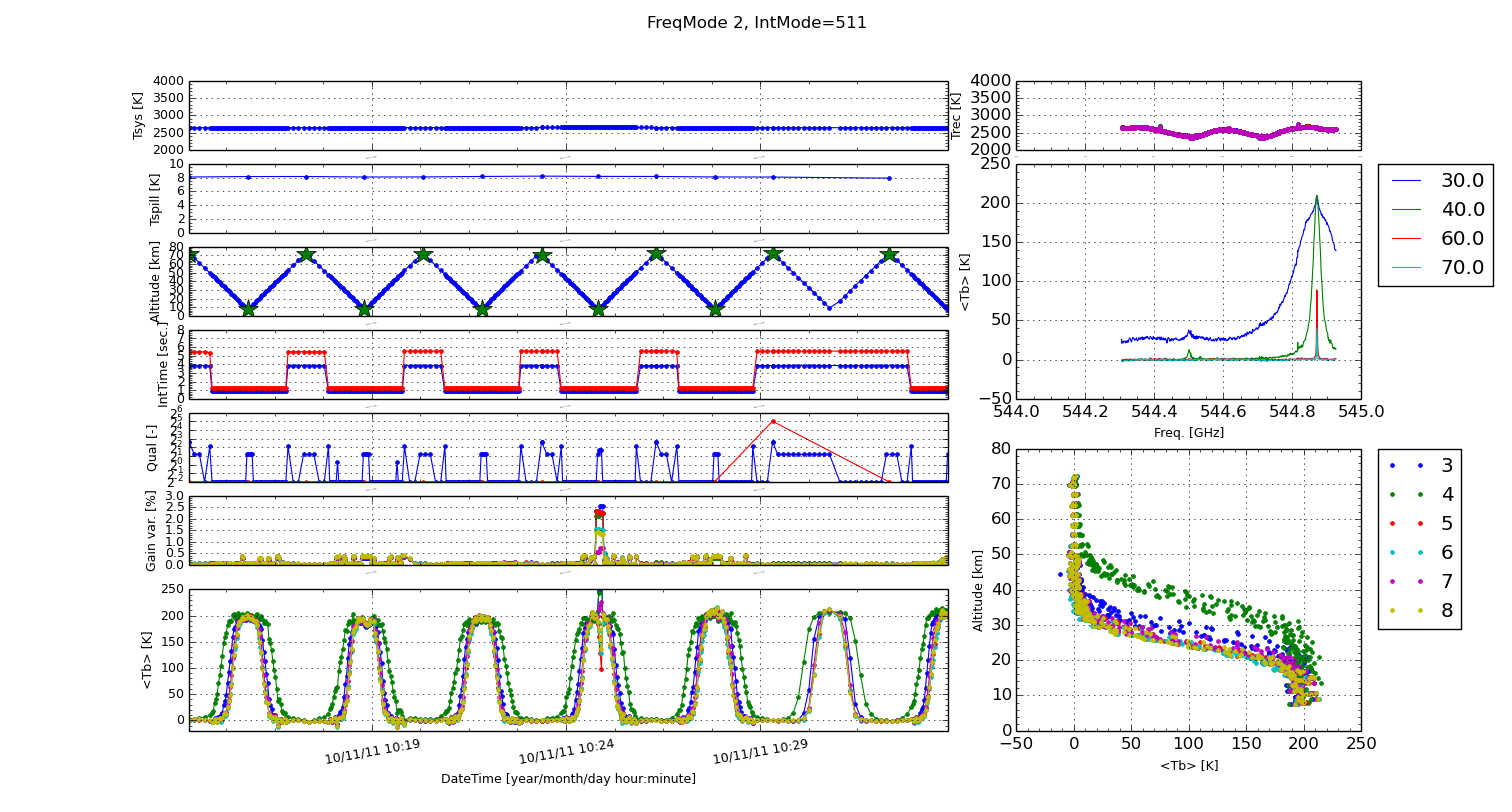
\includegraphics[width=14cm]{quality_control.png}
\caption{Quality flag description.}
\label{fig:quality}
\end{figure}

Quality related to a scan:\\
    1. check Tspill  - outside of valid range \\
    2. check Trec    - outside of valid range \\
    3. check Int     - corrupt integration time \\
    4. check Noise   - outside of valid range \\
    5. check Hotload - temperature data missing or out of range \\        
    6. check Scan    - corrupt scanning (tangent altitude is not  
                            decreasing or increasing as expected) \\ 
    7. check nr of atmospheric spectra in scan\\
    8. check observation sequence - Check that each atmospheric spectrum in the 
       scan is surrounded by reference measurements from sky beam 1.
       Accept n deviations for highest quality \\


Quality related to individual spectrum:\\
    1. Tb        - outside of valid range (-x -- 300\,K) or strange pattern \\
    2. Ref       - observation sequence - atmospheric spectrum is not collected 
                   between two sky beam 1 references\\
    3. Ref       - surrounding references have different integration times \\
    4. Ref       - high zerolag difference between surrounding references  \\
    5. Attitude  - high pointing error (maybe not relevant as error describes 
                   difference bteween target and achieved ) \\




\chapter{Summary}

text ...


